\chapter{Третья глава. Программная реализация моделей}
\label{cha:ch_3}
\section{Общая схема вычислений}

\par
В рассмотренных далее примерах рассматривалась вероятностная реализация алгоритмов CFR и MCCFR. При использовании метода MCCFR значения случайных событий генерируются перед началом каждой обучающей итерации. Данный подход позволяет сократить обьем памяти и ускорить вычисления в некоторых случаях\cite{MCCFR}.
При реализации примеров были выделены следующие компоненты:
\begin{itemize}
	\item описание правил игры (зависит от настроек);
	\item модуль с реализацией алгоритма относительно определенных правил.
\end{itemize}
\par
Настройки игры, например, по возможности могут включать число игроков, параметры выплат и т.п.
\par
Правила игры включают структуру игрового дерева, механизм распределения событий и функцию выплат. Игровое дерево строится с применением узлов -- обьектов с информацией о историии игры, о игроке и о возможных действиях.
\par
Итерации алгоритма проходят рекурсивно, начиная с вершины дерева. В ходе одной итерации t + 1 происходит следующее:
\begin{itemize}
\item расчет стратегий $q^{t + 1}$ используя контрафактические сожаления $t$(1.8);
\item расчет $t + 1$ слагаемого контрафактических сожалений;
\item обновление сумм контрафактических сожалений (1.7).
\end{itemize}
\par
Сам расчет итераций CFR происходит на основе определенных для каждого конкретного случая правил игры. Работа алгоритма начинается с создания игрового дерева. Далее происходит расчет заданного числа итераций. После любой итерации можно получить стратегии игроков, которые представляют из себя приближенное коррелированное равновесие.

\section{Моделирование раскрытия совместного преступления}

Рассмотрим несколько частных случаев задачи разоблачения совместного преступления. В соответствии с определением \ref{def1}, опишем игровые истории и информационные наборы игроков.
\begin{align*}
	A = \{\text{Предложить взятку}, \text{Не предлагать взятку}, \text{Принять взятку}, \\ \text{Отклонить взятку}, \text{Провести проверку}, \text{Не проводить проверку} \}
\end{align*}
Также определим перечень всех досупных игровых историй, включая терминальные:
\begin{align*}
hB = & \{\text{Предложить взятку}\}, \\
hBT = & \{\text{Предложить взятку}, \text{Принять взятку}\}, \\
zBTC = & \{\text{Предложить взятку}, \text{Принять взятку}, \text{Провести проверку}\}, \\
zBTnC = & \{\text{ Предложить взятку}, \text{Принять взятку}, \text{Не проводить проверку}\}, \\
hBnT = & \{ \text{Предложить взятку}, \text{Отклонить взятку} \}, \\
zBnTC = & \{\text{ Предложить взятку}, \text{Отклонить взятку}, \text{Провести проверку}\}, \\
zBnTnC = & \{\text{ Предложить взятку}, \text{Отклонить взятку}, \text{Не проводить проверку}\}, \\
hnB = & \{\text{ Не предлагать взятку}\}, \\
znBC = & \{\text{ Не предлагать взятку}, \text{Провести проверку}\}, \\
znBnC = & \{\text{ Не предлагать взятку}, \text{Не проводить проверку}\},
\end{align*}
\begin{equation*}
	H = \{\emptyset, hB, hBT, zBTC, zBTnC, hBnT, zBnTC, zBNCnC, hnB, znBC, znBnC\},
\end{equation*}
\begin{equation}
Z = \{zBTC, zBTnC, zBnTC, zBnTnC, znBC, znBnC\}.
\end{equation}
\par
Будем рассматривать множество $N$, состоящее из трех игроков: клиент, чиновник и инспектор
\begin{equation*}
N = \{0, 1, 2\}
\end{equation*}
Далее, определим информационные состояния игроков. В данном случае информационные наборы каждого игрока состоят из одного информационного состояния
\begin{align*}
\mathcal{I}_0 = & \{\{\emptyset\}\} \\
\mathcal{I}_1 = & \{\{hB\}\} \\
\mathcal{I}_2 = & \{\{hBT, hBnT, hnB\}\}
\end{align*}
\par
Данное определение информационных состояний позволяет сопоставить игроков и различные игровые истории и таким образом определить функцию $P$.

$$P(h0) = 0$$
$$P(hB)=1$$
$$P(hBT)=P(hBnT)=P(hnB)=2$$

Наконец, определим следующие терминальные выплаты для игроков из $N$ на множестве $Z$. В таблице \ref{tbl:u1} указано значение функции $u_i(z)$, для игрока $i \in N$ и терминальной истории $z \in Z$.

\begin{table}[H]
	\centering
	\begin{tabular}[t]{|c|c|c|c|c|c|c|}
		\hline
		$u$ &	$zBTC$ & $zBTnC$ &	$zBnTC$ & $zBnTnC$ & $znBC$ & $znBnC$ \\
		\hline
		$0$	&$v-b-p_L-p_H$&	$v-b$&	$-p_L$&	$0$&	$0$ &	$0$ \\
		\hline
		$1$&	$b-q$&	$b$&	$r$&	$r$&	$0$&	$0$ \\
		\hline
		$2$&	$x+\Delta x$&	$x$&	$y+\Delta y$&	$y$&	$z$&	$z+\Delta z$ \\
		
		\hline
	\end{tabular}
	\caption{\centering Значения функции выплат $u$}
	\label{tbl:u1}
\end{table}

Проведем расчеты для некоторых значений параметров. Рассмотрим набор параметров из таблицы \ref{tbl:s1_1} и проведем расчет равновесия для данного случая

\begin{table}[H]
	\centering
	\begin{tabular}[t]{|c|c|c|c|c|c|c|c|c|c|c|c|}
		\hline
		$v$ &	$b$ & $p_L$ &	$p_H$ & $q$ & $r$ & $\Delta x$ & $x$ & $\Delta y$ & $y$ & $\Delta z$ & $z$ \\
		\hline
		6 &	4 & 3 &	3 & 5 & 1 & 6 & -3 & 4 & -2 & 2 & -1 \\
		\hline
	\end{tabular}
\caption{\centering Значения параметров для первого примера}
\label{tbl:s1_1}
\end{table}
\par
Учитывая параметры из таблицы \ref{tbl:s1_1} построим игровое дерево со случайным профилем стратегий. Схематичное изображение игрового дерева показано на рисунке \ref{fig:c3th11}.

\begin{figure}[H]
	\centering
	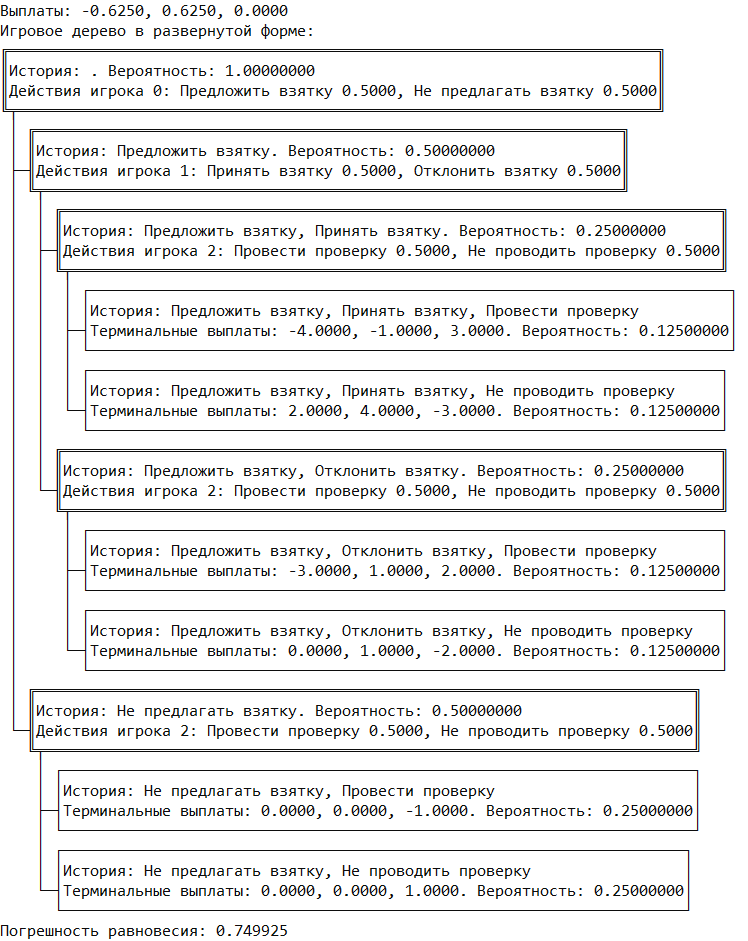
\includegraphics[width=0.9\linewidth]{inc/img/c3th11}
	\caption{Дерево игры с первой группой параметров. Случайные стратегии}
	\label{fig:c3th11}
\end{figure}

\par
На рисунке \ref{fig:c3th11} прямоугольными элементами отмечены все игровые истории, начиная с начала игры. Ребра между элементами обозначают возможные переходы между игровыми историями. Каждой нетерминальной игровой истории соответствует перечень доступных действий и стратегия их выбора. Терминальные истории сопровождаются информацией о выплатах игрокам. Для каждой истории указывается вероятность ее реализации. Расчетная эксплуатируемость данного профиля стратегий составляет примерно $0.75$. Для достижения этого значения инспектору достаточно проводить проверку с вероятностью $1.0$, изменив тем самым свой ожидаемый выигрыш с $0$ до $0.75$. Данный стратегический профиль достаточно далек от равновесия.
\par
Попробуем улучшить стратегический профиль. Проведем $T=10000$ обучающих итераций алгоритма на данном игровом дереве. Информация о обновленном стратегическом профиле представлена на рисунке \ref{fig:c3th12}.
\begin{figure}[H]
	\centering
	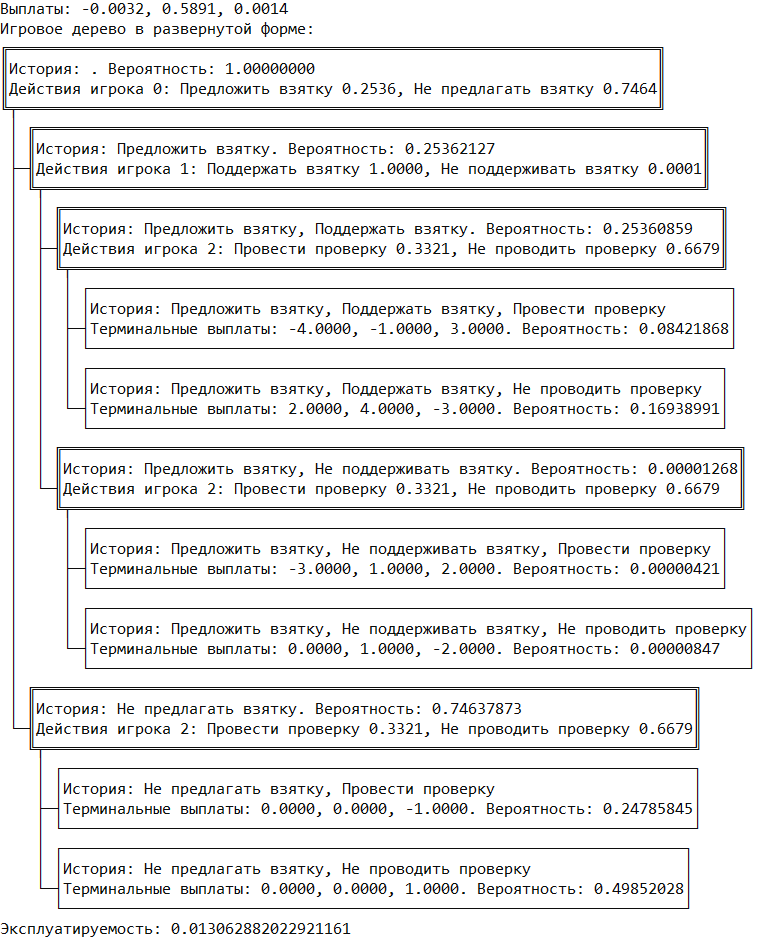
\includegraphics[width=0.9\linewidth]{inc/img/c3th12}
	\caption{Дерево игры с первой группой параметров. $T = 10000$}
	\label{fig:c3th12}
\end{figure}
\par
На рисунке \ref{fig:c3th12} отмечены выплаты, измененные стратегии игроков и измененные вероятности достижения различных игровых историй. Как можно заметить, погрешность равновесия снизилась до порядка $0.01$, что сопоставимо с оценкой из теоремы \ref{CfrTStrategyExp}.
\par
Дальнейшее увеличение числа итераций приводит к уменьшению погрешности равновесия. График изменения расчетной погрешности равновесия для данного примера приведен на рисунке \ref{fig:c3e1}.

\begin{figure}[H]
	\centering
	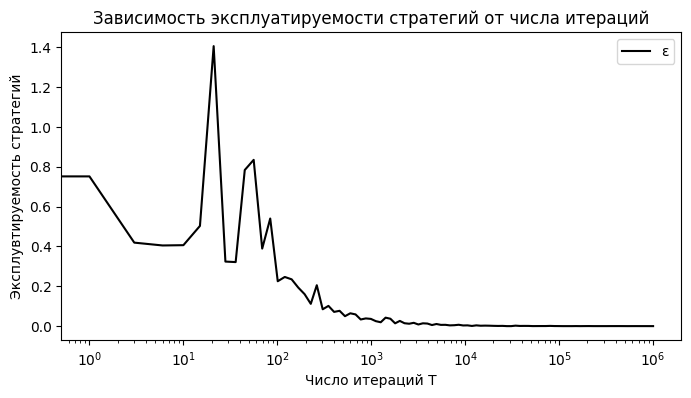
\includegraphics[width=0.8\linewidth]{inc/img/c3e1}
	\caption{Расчетная эксплуатируемость стратегий в зависимости от $T$}
	\label{fig:c3e1}
\end{figure}

\par
Рассмотрим другой набор параметров алгоритма (Таблица \ref{tbl:s1_2}).
\begin{table}[H]
	\centering
	\begin{tabular}[t]{|c|c|c|c|c|c|c|c|c|c|c|c|}
		\hline
		$v$ &	$b$ & $p_L$ &	$p_H$ & $q$ & $r$ & $\Delta x$ & $x$ & $\Delta y$ & $y$ & $\Delta z$ & $z$ \\
		\hline
		12 &	3 & 8 &	8 & 4 & 2 & 9 & 1 & 1 & 7 & 3 & 5 \\
		\hline
	\end{tabular}
	\caption{\centering Значения параметров для второго примера}
	\label{tbl:s1_2}
\end{table}
\par
Построим игровую модель и проведем $10000$ обучающих итераций. Полученный профиль стратегий представлен на рисунке \ref{fig:c3th21}.
\begin{figure}[H]
	\centering
	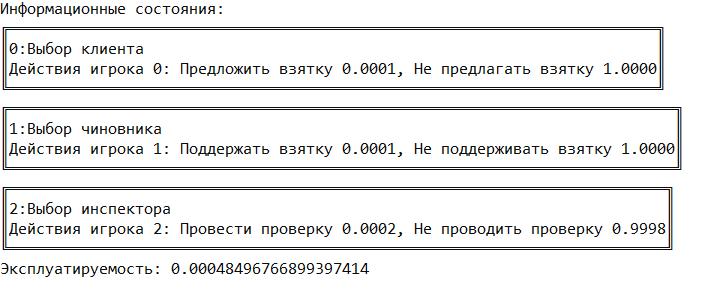
\includegraphics[width=0.8\linewidth]{inc/img/c3th21}
	\caption{Стратегии игроков для второго примера. $T=10000$}
	\label{fig:c3th21}
\end{figure}
\par
В результате мы получили профиль, который состоит из чистых стратегий. Хотя данное решение и является равновесием, оно маловероятно на практике по интуитивным соображениям. Так как алгоритм предоставляет единственное решение, имеет смысл наложить дополнительные ограничения на рассматриваемую задачу. Попробуем получить дополнительную информацию о данной игре. Для этого попробуем зафиксировать стратегию одного игрока и найти равновесие для двух оставшихся. Таким образом, найдем зависимости $\beta$ и $\gamma$ от $\alpha$, $\alpha$ и $\gamma$ от $\beta$ и зависимость $\alpha$ и $\beta$ от $\gamma$. Графики соответствующих зависимостей представлены на рисунках .

\begin{figure}[H]
	\centering
	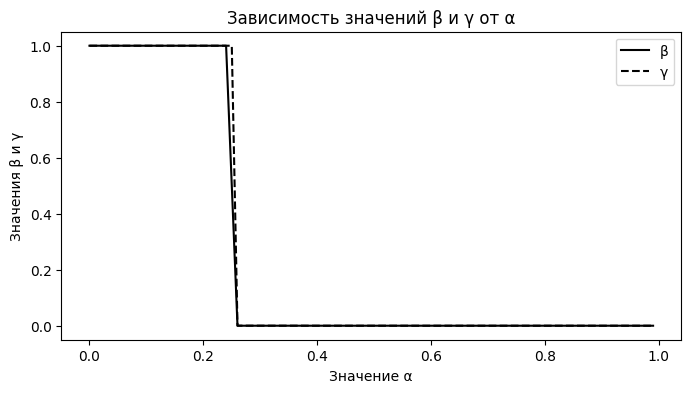
\includegraphics[width=0.8\linewidth]{inc/img/c3ex2alpha}
	\caption{График зависимости $ \beta$ и $ \gamma$ от $ \alpha$}
	\label{fig:c3ex2alpha}
\end{figure}

\begin{figure}[H]
	\centering
	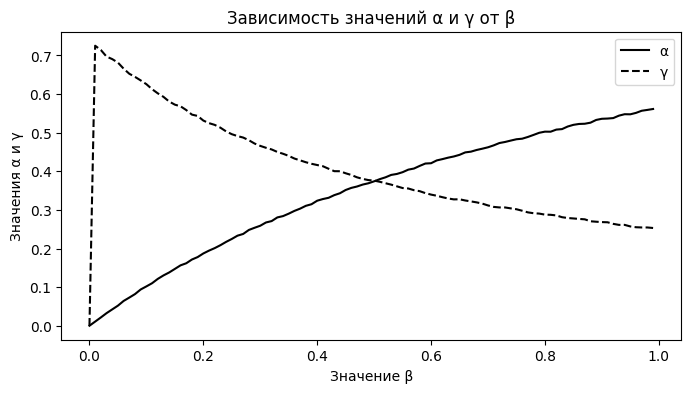
\includegraphics[width=0.8\linewidth]{inc/img/c3ex2beta}
	\caption{График зависимости $\alpha $ и $ \gamma$ от $ \beta$}
	\label{fig:c3ex2beta}
\end{figure}

\begin{figure}[H]
	\centering
	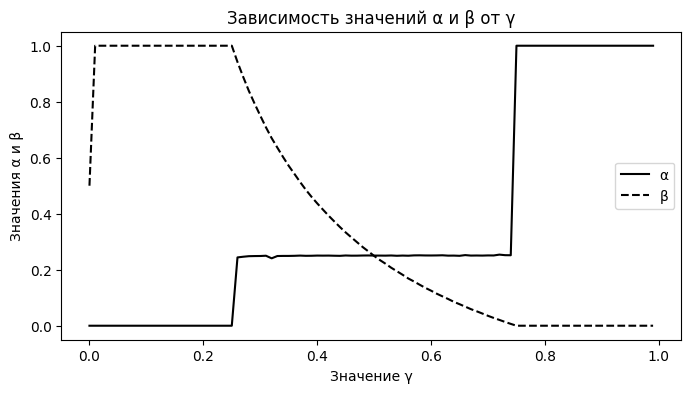
\includegraphics[width=0.8\linewidth]{inc/img/c3ex2gamma}
	\caption{График зависимости $\alpha $ и $ \beta$ от $ \gamma$}
	\label{fig:c3ex2gamma}
\end{figure}

\par
В соответствии с оценкой (\ref{eq:2.5}), вероятность проверки $\alpha$ влияет на решение чиновника о принятии взятки. В данном случае, критическое значение равно $0.25$, и на графиках \ref{fig:c3ex2alpha} и \ref{fig:c3ex2gamma} прослеживается изменение поведения участников при его преодолении инспектором.
\section{Моделирование коррупции в иерархической структуре}

В данной работе в качестве основного объекта исследования была выбрана модель коррупции в иерархической структуре. Рассмотрим частный случай параметров иерархии, которые описаны в (\ref{eq2.9}). Как и в предыдущем примере, опишем игровые истории и информационные наборы игроков.
\begin{align*}
	A = \{\text{НеCовКр}, \text{СовКр}, \text{НеПровСот}, \text{ПровСот}, \text{ПредлВз}, \text{ВыплШт},\\ \text{РазРук}, \text{ПринВз}, \text{ОтклВз}, \text{ПровЧин}, \text{НеПровЧин} \}
\end{align*}
Стоит отметить, что приведенный набор действий не содержит отдельные действия для проверки первого и второго сотрудника. Вместо этого будет использоваться решение о проверке каждого или переход к следующему.
Далее, определим перечень всех досупных игровых историй без терминальных:

$$	h_{1} = \{\text{НеПровЧин}\}, \;\; h_{2} = \{\text{НеПровЧин}, \text{СовКр}\}, \;\; h_{3} = \{\text{НеПровЧин}, \text{СовКр}, \text{СовКр}\}, $$
$$	h_{4} = \{\text{НеПровЧин}, \text{СовКр}, \text{СовКр}, \text{ПровСот}\}, $$
$$	h_{5} = \{\text{НеПровЧин}, \text{СовКр}, \text{СовКр}, \text{ПровСот}, \text{ПредлВз}\}, $$
$$	h_{6} = \{\text{НеПровЧин}, \text{СовКр}, \text{СовКр}, \text{НеПровСот}\}, $$
$$	h_{7} = \{\text{НеПровЧин}, \text{СовКр}, \text{СовКр}, \text{НеПровСот}, \text{ПровСот}\}, $$
$$	h_{8} = \{\text{НеПровЧин}, \text{СовКр}, \text{СовКр}, \text{НеПровСот}, \text{ПровСот}, \text{РазРук}\}, $$
$$	h_{9} = \{\text{НеПровЧин}, \text{СовКр}, \text{СовКр}, \text{НеПровСот}, \text{ПровСот}, \text{РазРук}, \text{ПредлВз}\}, $$
$$	h_{10} = \{\text{НеПровЧин}, \text{СовКр}, \text{СовКр}, \text{НеПровСот}, \text{ПровСот}, \text{ПредлВз}\}, $$
$$	h_{11} = \{\text{НеПровЧин}, \text{СовКр}, \text{СовКр}, \text{НеПровСот}, \text{НеПровСот}\}, $$
$$	h_{12} = \{\text{НеПровЧин}, \text{СовКр}, \text{НеCовКр}\},\;\;h_{13} = \{\text{НеПровЧин}, \text{СовКр}, \text{НеCовКр}, \text{ПровСот}\} $$
$$	h_{14} = \{\text{НеПровЧин}, \text{СовКр}, \text{НеCовКр}, \text{ПровСот}, \text{ПредлВз}\}, $$
$$	h_{15} = \{\text{НеПровЧин}, \text{СовКр}, \text{НеCовКр}, \text{НеПровСот}\}, $$
$$	h_{16} = \{\text{НеПровЧин}, \text{НеCовКр}\},\;\;h_{17} = \{\text{НеПровЧин}, \text{НеCовКр}, \text{СовКр}\}, $$
$$	h_{18} = \{\text{НеПровЧин}, \text{НеCовКр}, \text{СовКр}, \text{НеПровСот}\}, $$
$$	h_{19} = \{\text{НеПровЧин}, \text{НеCовКр}, \text{СовКр}, \text{НеПровСот}, \text{ПровСот}\}, $$
$$	h_{20} = \{\text{НеПровЧин}, \text{НеCовКр}, \text{СовКр}, \text{НеПровСот}, \text{ПровСот}, \text{ПредлВз}\}, $$
$$	h_{21} = \{\text{НеПровЧин}, \text{НеCовКр}, \text{НеCовКр}\}, $$
$$	h_{22} = \{\text{НеПровЧин}, \text{НеCовКр}, \text{НеCовКр}, \text{НеПровСот}\}, $$
$$	h_{23} = \{\text{ПровЧин}\}, \;\; h_{24} = \{\text{ПровЧин}, \text{СовКр}\}, \;\; h_{25} = \{\text{ПровЧин}, \text{СовКр}, \text{СовКр}\}, $$
$$	h_{26} = \{\text{ПровЧин}, \text{СовКр}, \text{СовКр}, \text{ПровСот}\}, $$
$$	h_{27} = \{\text{ПровЧин}, \text{СовКр}, \text{СовКр}, \text{ПровСот}, \text{ПредлВз}\}, $$
$$	h_{28} = \{\text{ПровЧин}, \text{СовКр}, \text{СовКр}, \text{НеПровСот}\}, $$
$$	h_{29} = \{\text{ПровЧин}, \text{СовКр}, \text{СовКр}, \text{НеПровСот}, \text{ПровСот}\}, $$
$$	h_{30} = \{\text{ПровЧин}, \text{СовКр}, \text{СовКр}, \text{НеПровСот}, \text{ПровСот}, \text{РазРук}\}, $$
$$	h_{31} = \{\text{ПровЧин}, \text{СовКр}, \text{СовКр}, \text{НеПровСот}, \text{ПровСот}, \text{РазРук}, \text{ПредлВз}\}, $$
$$	h_{32} = \{\text{ПровЧин}, \text{СовКр}, \text{СовКр}, \text{НеПровСот}, \text{ПровСот}, \text{ПредлВз}\}, $$
$$	h_{33} = \{\text{ПровЧин}, \text{СовКр}, \text{СовКр}, \text{НеПровСот}, \text{НеПровСот}\}, $$
$$	h_{34} = \{\text{ПровЧин}, \text{СовКр}, \text{НеCовКр}\},\;\;h_{35} = \{\text{ПровЧин}, \text{СовКр}, \text{НеCовКр}, \text{ПровСот}\} $$
$$	h_{36} = \{\text{ПровЧин}, \text{СовКр}, \text{НеCовКр}, \text{ПровСот}, \text{ПредлВз}\}, $$
$$	h_{37} = \{\text{ПровЧин}, \text{СовКр}, \text{НеCовКр}, \text{НеПровСот}\}, $$
$$	h_{38} = \{\text{ПровЧин}, \text{НеCовКр}\},\;\;h_{39} = \{\text{ПровЧин}, \text{НеCовКр}, \text{СовКр}\}, $$
$$	h_{40} = \{\text{ПровЧин}, \text{НеCовКр}, \text{СовКр}, \text{НеПровСот}\}, $$
$$	h_{41} = \{\text{ПровЧин}, \text{НеCовКр}, \text{СовКр}, \text{НеПровСот}, \text{ПровСот}\}, $$
$$	h_{42} = \{\text{ПровЧин}, \text{НеCовКр}, \text{СовКр}, \text{НеПровСот}, \text{ПровСот}, \text{ПредлВз}\}, $$
$$	h_{43} = \{\text{ПровЧин}, \text{НеCовКр}, \text{НеCовКр}\}, $$
$$	h_{44} = \{\text{ПровЧин}, \text{НеCовКр}, \text{НеCовКр}, \text{НеПровСот}\}, $$
\begin{equation}
	\label{HmZ2}
	H \setminus Z = \{\emptyset, h_{1}, \dots , h_{44}\}.
\end{equation}

\par
Терминальные истории подобного примера приведены в главе 2. Будем рассматривать множество $N$, состоящее из четырех игроков: сотрудник $C_0$, сотрудник $C_1$, чиновник $O$ и инспектор $I$
\begin{equation*}
	N = \{0, 1, 2, 3\}
\end{equation*}
Далее, определим информационные состояния игроков. В данном случае информационные наборы некотрых игроков состоят из нескольких информационных состояний

 $$	I_1 = \{\emptyset\},\; I_2 = \{h_{1},\; h_{23}\},\;	I_3 = \{h_{2},\; h_{16},\; h_{h24},\; h_{38}\},  $$
 $$	I_4 = \{h_{3},\;h_{12},\;h_{17},\;h_{21},\;h_{25},\;h_{34},\;h_{39},\;h_{43}\}, $$
 $$	I_5 = \{h_{6},\;h_{15},\;h_{18},\;h_{22},\;h_{28},\;h_{37},\;h_{40},\;h_{44}\}, $$
 $$	I_6 = \{h_{4},\;h_{13},\;h_{26},\;h_{35}\},\; I_7 = \{h_{h8},\; h_{30}\},$$
 $$	I_8 = \{h_{9},\;h_{31}\},\;I_9 = \{h_{5},\;h_{14},\;h_{27},\;h_{36}\},  $$
 $$	I_{10} = \{h_{7},\;h_{h_19},\;h_{29},\;h_{41}\},\;I_{11} = \{h_{10},\;h_{20},\;h_{32},\;h_{42}\}, $$
 $$	\mathcal{I}_0 = \{I_2,\;I_6,\;I_7\},  $$
 $$	\mathcal{I}_1 = \{I_3,\;I_{10}\},  $$
 $$	\mathcal{I}_2 = \{I_4,\;I_5,\;I_8,\;I_9,\;I_{11}\},  $$
 $$	\mathcal{I}_3 = \{I_1\}. $$
\par
Данное определение информационных состояний позволяет сопоставить игроков и различные игровые истории.

Функцию $u_i(z)$, для игрока $i \in N$ и терминальной истории $z \in Z$, определим  в соответствии с формой игры на рисунках \ref{fig:figef21} и \ref{fig:figef22}.

Проведем расчеты для некоторых значений параметров. Рассмотрим набор параметров из таблицы \ref{tbl:s2_1} и проведем расчет равновесия для данного случая

\begin{table}[H]
	\centering
	\begin{tabular}[t]{|c|c|c|c|c|c|c|c|c|c|c|c|c|c|c|}
		\hline
		$s_0$ & $b_0$ & $s_1$ & $b_1$ & $co$ & $ci$ & $fs$ &	$fb$ & $fq$ & $fns$ & $fe$ & $fbc$ & $rs$ & $rb$ & $rq$\\
		\hline
		 80 & 24 & 40 & 12 & 2 & 2 & 110 & 15 & 4 & 2 & 1 & 10 & 4 & 1 & 10\\
		\hline
	\end{tabular}
	\caption{\centering Значения параметров для примера}
	\label{tbl:s2_1}
\end{table}
\par
Учитывая параметры из таблицы \ref{tbl:s2_1} построим игровое дерево со случайным профилем стратегий. Схематичное изображение игрового дерева показано на рисунке \ref{fig:c3th11}.

\begin{figure}[H]
	\centering
	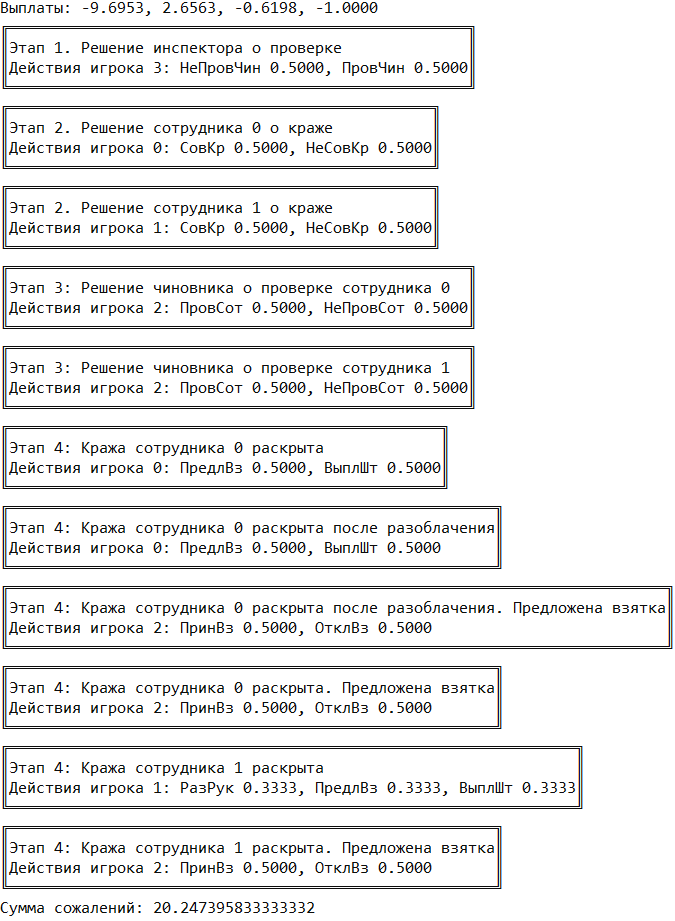
\includegraphics[width=0.8\linewidth]{inc/img/c32th11}
	\caption{Дерево игры с первой группой параметров. Случайные стратегии}
	\label{fig:c32th11}
\end{figure}

\par
На рисунке \ref{fig:c32th11} прямоугольными элементами отмечены все информационные состояния игроков. Каждому информационному состоянию соответствует перечень доступных действий и стратегия их выбора. Расчетная расчетная сумма сожалений всех игроков превосходит $20$ и данный стратегический профиль достаточно далек от равновесия и можно провести минимизацию сожалений.
\par
Попробуем улучшить стратегический профиль. Проведем $T=10000$ обучающих итераций алгоритма на данном игровом дереве. Информация о обновленном стратегическом профиле представлена на рисунке \ref{fig:c32th12}.
\begin{figure}[H]
	\centering
	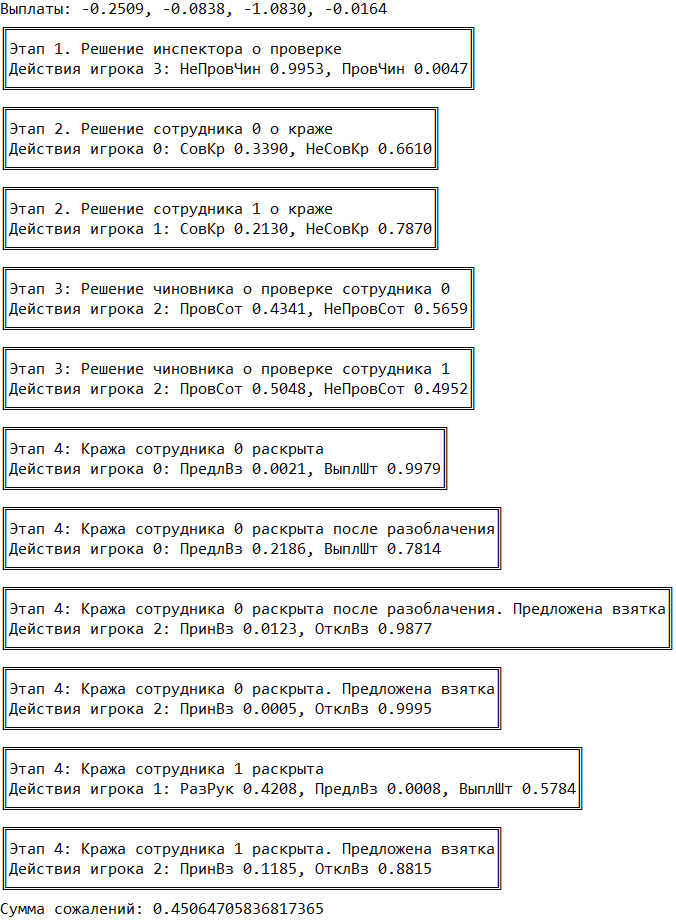
\includegraphics[width=0.8\linewidth]{inc/img/c32th12}
	\caption{Дерево игры с первой группой параметров. $T = 10000$}
	\label{fig:c32th12}
\end{figure}
\par
На рисунке \ref{fig:c32th12} отмечены измененные стратегии игроков. Как можно заметить, сумма сожалений снизилась до $0.38$. Дальнейшее увеличение числа итераций приводит к уменьшению суммы сожалений. График изменения чуммы сожалений для данного примера приведен на рисунке \ref{fig:c3r2}.

\begin{figure}[H]
	\centering
	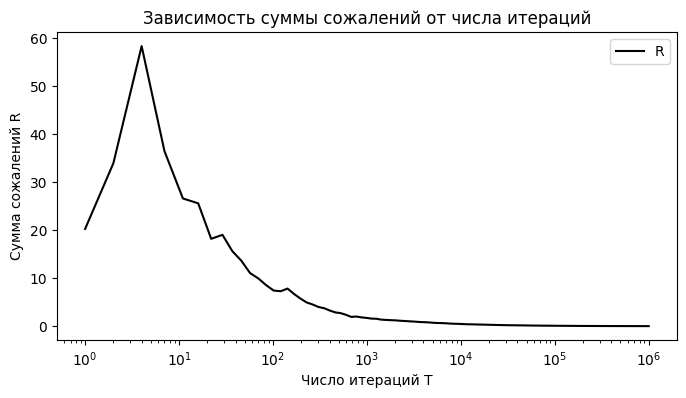
\includegraphics[width=0.8\linewidth]{inc/img/c3r2}
	\caption{Расчетная сумма сожалений в зависимости от $T$}
	\label{fig:c3r2}
\end{figure}